\documentclass[
english,
svgnames,
notes=hide,
% handout, % Uncomment to disable transitions and animations
12pt]{beamer}



% \usetheme{default}
% \usetheme{AnnArbor}
% \usetheme{Boadilla}
% \usetheme{CambridgeUS}
\usetheme{Madrid}
%
% \usecolortheme{beetle}
% \usecolortheme{dolphin}
% \usecolortheme{lily}
% \usecolortheme{whale}

\usefonttheme{default} % Typeset using the default sans serif font
\useinnertheme{circles}



\usepackage{soul}
\usepackage{amssymb,latexsym,amsmath}
\usepackage[mathscr]{euscript}
\usepackage{mathrsfs}
\usepackage{braket}
% \usecolortheme{beaver}

\date{10 December 2024}
\author[Mickael Kovel]{Mickael Kovel}
\title[ELEC-H-550]{Embedded System Security} % The short title in the optional parameter appears at the bottom of every slide, the full title in the main parameter is only on the title page

\subtitle{MAC Address Anonymization} % Presentation subtitle, remove this command if a subtitle isn't required


\institute[ULB]{Université Libre de Bruxelles \\ \smallskip \textit{}} % Your institution, the optional parameter can be used for the institution shorthand and will appear on the bottom of every slide after author names, while the required parameter is used on the title slide and can include your email address or additional information on separate lines
% \def\presentationtitle{Testing the black-hole area law with GW150914}


\beamertemplatenavigationsymbolsempty
\begin{document}

\begin{frame}
	\titlepage % Output the title slide, automatically created using the text entered in the PRESENTATION INFORMATION block above
\end{frame}

% \begin{frame}
% 	\frametitle{Programme} % Slide title, remove this command for no title

% 	\tableofcontents % Output the table of contents (all sections on one slide)
% 	%\tableofcontents[pausesections] % Output the table of contents (break sections up across separate slides)
% \end{frame}


%------------------------------------------------


\begin{frame}
  \section{Introduction}
  \frametitle{Introduction}
  \begin{itemize}
    \item The rise of connected devices in the Internet of Things (IoT) has led to the widespread collection of MAC addresses, which are used to identify devices on a network. \pause 
    \item While these addresses play a crucial role in network communication, they can also be exploited for tracking purposes, raising concerns about user privacy. \pause 
    \item This project explores the implications of MAC address usage from both a privacy and legal perspective, focusing on potential risks and protection mechanisms. \pause
    \item The goal is to understand how MAC addresses can be anonymized and what legal measures are in place to ensure data protection and respect for privacy.
  \end{itemize}
\end{frame}


\begin{frame}
  \section{What is a MAC Address?}
  \frametitle{What is a MAC Address?}
  \begin{itemize}
    \item Device identification on a network \pause
      \begin{itemize}
        \item Using MAC addresses to identify devices \pause
        \item Similar to postal addresses for identifying houses \pause
        \item Enables communication on a network segment \pause
      \end{itemize}
    \item Definition \pause
      \begin{itemize}
        \item A unique identifier assigned to a network interface controller (NIC) \pause
        \item Used for communication within a network 
      \end{itemize}
  \end{itemize}
\end{frame}

\begin{frame}
  \section{How is a MAC Address Provided?}
  \frametitle{How is a MAC Address Provided?}
  \begin{itemize}
    \item Provided by the manufacturer of the network interface controller (NIC) \pause
    \item Typically assigned at the factory and hardcoded into the hardware \pause
    \item Cannot be changed by the user \pause
    \item Ensures global uniqueness 
  \end{itemize}
\end{frame}

\begin{frame}
  \section{What is the Structure of a MAC Address?}
  \frametitle{What is the Structure of a MAC Address?}
	\begin{figure}
    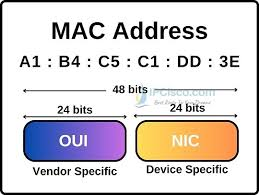
\includegraphics[width=0.5\linewidth]{pictures/mac.jpeg}
		\caption{MAC Address Structure}
	\end{figure}
\end{frame}


\begin{frame}
  \section{What is the Structure of a MAC Address?}
  \frametitle{What is the Structure of a MAC Address?}
  \begin{itemize}
    \item 48 bits long, represented by a 12-digit hexadecimal number \pause
    \item First part: OUI (Organizationally Unique Identifier) \pause
      \begin{itemize}
        \item Identifies the NIC manufacturer \pause
        \item Composed of 24 bits (6 hexadecimal digits) \pause
      \end{itemize}
    \item Second part: Device Identifier \pause
      \begin{itemize}
        \item Assigned by the manufacturer, unique to each device \pause
        \item Composed of 24 bits (6 hexadecimal digits) 
      \end{itemize}
  \end{itemize}
\end{frame}

\begin{frame}
  \section{Bluetooth and MAC Addresses}
  \frametitle{Bluetooth and MAC Addresses}
  \begin{itemize}
    \item Bluetooth devices use a 48-bit Bluetooth device address (BD ADDR) \pause
    \item Similar to a MAC address, but specifically for Bluetooth devices \pause
    \item BD ADDRs are also unique and can be used to track devices 
  \end{itemize}
\end{frame}

\begin{frame}
  \section{Privacy Implications of a MAC Address}
  \frametitle{Privacy Implications of a MAC Address}
  \begin{itemize}
    \item MAC addresses can be used to track devices on a network \pause
    \item Privacy issues arise if MAC addresses are exposed \pause
    \item Privacy protection techniques, such as MAC address anonymization 
  \end{itemize}
\end{frame}

\begin{frame}
  \section{Where Are MAC Addresses Used?}
  \frametitle{Where Are MAC Addresses Used?}
  \begin{itemize}
    \item Wi-Fi and Ethernet networks \pause
      \begin{itemize}
        \item Used to identify devices on a local network \pause
        \item Associated with IP addresses using the ARP protocol
      \end{itemize}
    % \item Used in data exchanges \pause
    %   \begin{itemize}
    %     \item Helps route data packets to the correct destination 
    %   \end{itemize}
  \end{itemize}
\end{frame}

% \begin{frame}
%   \section{What Does the Law Say?}
%   \frametitle{What Does the Law Say?}
%   \begin{itemize}
%     \item Role of MAC addresses in the network \pause
%       \begin{itemize}
%         \item Using MAC addresses to identify devices on the network 
%       \end{itemize}
%   \end{itemize}
% \end{frame}

\begin{frame}
  \section{What Does the Law Say?}
  \pause
  \frametitle{What Does the Law Say?}
	\begin{quote}
    \begin{block}{GDPR}
    ``
  The principles of data protection should apply to any information concerning an
  identified or identifiable natural person. [...]
  \ul{The principles of data protection should therefore not apply to anonymous information}, [...]
  ``
\end{block}
  \end{quote}
\end{frame}

\begin{frame}
  \section{What Does the Law Say?}
  \frametitle{What Does the Law Say?}
  \begin{quote}
    \begin{block}{European Convention on Human Rights}
  \begin{enumerate}
\item[35.] ``Admissibility criteria
\end{enumerate}
  \begin{enumerate}
    \item[1.] [...]
    \item[2.] \ul{The Court shall not deal with any application submitted under Article 34 that}
    \begin{enumerate}
      \item[•] \ul{is anonymous}; or [...]
        ``
    \end{enumerate}
  \end{enumerate}
\end{block}
  \end{quote}
\end{frame}

\begin{frame}
  \section{What Does the Law Say?}
  \frametitle{What Does the Law Say?}
  \begin{quote}
    \begin{block}{Convention 108+}
    \begin{enumerate}
      \item[18.] ``
    [...]{The use of a pseudonym or of any digital identifier/
    digital identity does not lead to anonymisation of 
  the data}[...]
    ``
  \item[19.] ``{Data is to be considered as anonymous only as
    long as it is impossible to re-identify the data subject
    or if such re-identification would require unreasonable
  time, effort or resources}[...], 
    ``
  \item[20.] ``When data is made anonymous, appropriate
    means should be put in place to avoid re-identification
  of data subjects,[...]
    ``
    \end{enumerate}
    \end{block}
  \end{quote}
\end{frame}

\begin{frame}
  \section{What Does the Law Say?}
  \frametitle{What Does the Law Say?}
  \begin{quote}
    \begin{block}{Belgian Law on Data Protection}
  ``
  Articles 101, 134, and 164 of the Belgian Act of 30 July 2018 on the protection
  of individuals with regard to the processing of personal data
  stipulate that the personal data referred to in
  \ul{Articles 99, 132, and 162 must be anonymized before they can be accessed.} 
  These articles primarily concern the processing of personal data for historical, 
  scientific, or statistical purposes.
  ``
  \end{block}
  \end{quote}
\end{frame}

\begin{frame}
  \section{What Are the Risks Related to MAC Address?}
  \frametitle{Risks Related to MAC Address}
  \begin{itemize}
    \item \textbf{Tracking} \pause
    \item \textbf{Audience Measurement} \pause
    \item \textbf{Profiling} \pause
    \item \textbf{Re-identification} \pause
    \item \textbf{Spoofing} 
  \end{itemize}
\end{frame}

\begin{frame}
  \section{Who Can Access a MAC Address?}
  \frametitle{Who Can Access a MAC Address?}
  \begin{itemize}
    \item \textbf{Anyone can access a MAC address.} It is transmitted in clear text and can be easily intercepted with the right tools. \pause
    \item The main risk arises when a MAC address is tied to a specific location or time, such as connecting to a Wi-Fi network. \pause
    \item The privacy risk increases when this data is recorded over time, enabling the tracking of individuals. 
  \end{itemize}
\end{frame}

\begin{frame}
  \section{Internet Service Providers}
  \frametitle{Internet Service Providers (ISPs)}
  \begin{itemize}
    \item ISPs can access MAC addresses when users connect to their network. \pause
    \item ISPs have access to all data passing through their network, including MAC addresses. \pause
    \item This data can be used for network management, troubleshooting, and advertising. \pause
    \item The use of MAC addresses for tracking or profiling purposes is generally prohibited under data protection regulations. 
  \end{itemize}
\end{frame}

\begin{frame}
  \section{Audience Measurement}
  \frametitle{Audience Measurement Companies}
  \begin{itemize}
    \item MAC addresses can be collected by audience measurement companies using Wi-Fi sensors in public spaces. \pause
    \item This data is used to measure foot traffic and assess advertising effectiveness. \pause
    \item The use of this data is regulated by data protection laws, and it must be anonymized to protect user privacy. \pause
    \item Concerns arise when data is used for unethical purposes, such as surveillance or tracking without consent. 
  \end{itemize}
\end{frame}

\begin{frame}
  \section{Profiling}
  \frametitle{Profiling Using MAC Addresses}
  \begin{itemize}
    \item MAC addresses allow the creation of detailed user profiles by correlating data such as connection times, locations, and usage patterns. \pause
    \item This information can reveal personal habits, routines, and preferences. \pause
    \item Companies use this data for targeted advertising, while malicious actors may exploit it for social engineering attacks. \pause
    \item This type of profiling is often invisible to users but constitutes a significant invasion of privacy. 
  \end{itemize}
\end{frame}

\begin{frame}
  \section{Re-identification}
  \frametitle{Re-identification Risks}
  \begin{itemize}
    \item Even randomized MAC addresses can be re-identified when combined with other data sources. \pause
    \item Usage patterns such as connection duration or frequency can link a temporary address to its original one. \pause
    \item This compromises the effectiveness of anonymization and exposes users to risks if data is leaked or poorly secured. 
  \end{itemize}
\end{frame}

\begin{frame}
  \section{Spoofing}
  \frametitle{MAC Address Spoofing}
  \begin{itemize}
    \item Spoofing allows attackers to falsify their MAC address to bypass network access controls or steal identities. \pause
    \item This is particularly dangerous in systems reliant on MAC addresses for security, such as IoT devices. \pause
    \item Spoofing illustrates the limitations of using MAC addresses as secure identifiers. 
  \end{itemize}
\end{frame}

\begin{frame}
  \section{How to Anonymize a MAC Address?}
  \frametitle{Anonymizing a MAC Address}
  \begin{itemize}
    \item \textbf{Truncation} \pause
    \item \textbf{Hashing} \pause
    \item \textbf{Encryption} 
  \end{itemize}
\end{frame}

\begin{frame}
  \section{Truncation}
  \frametitle{Truncation}
  Truncation involves shortening the MAC address by keeping only part of it, such as the first 6 octets (manufacturer's identifier), or a random portion.
  \begin{itemize}
    \item \textbf{Advantages:} \pause
      \begin{itemize}
        \item Simple to implement. \pause
        \item Reduces the risk of re-identification as the remaining portion doesn't contain enough identifying information. \pause
      \end{itemize}
    \item \textbf{Disadvantages:} \pause
      \begin{itemize}
        \item Loss of information if finer identification is needed. \pause
        \item May not be sufficient for higher anonymity as the remaining address part may still enable tracing. 
      \end{itemize}
  \end{itemize}
\end{frame}

\begin{frame}
  \section{Hashing}
  \frametitle{Hashing}
  Hashing applies a mathematical function to the MAC address, producing a fixed-size output (hash). The process is irreversible.
  \begin{itemize}
    \item \textbf{Advantages:} \pause
      \begin{itemize}
        \item Irreversible, meaning the original MAC address cannot be recovered. \pause
        \item Protection against rainbow table attacks with the use of salt. \pause
        \item Easy to implement when access to the original MAC address is not needed post-anonymization. \pause
      \end{itemize}
    \item \textbf{Disadvantages:} \pause
      \begin{itemize}
        \item Loss of the original MAC address, which may be problematic if recovery is required for auditing or re-identification. \pause
      \end{itemize}
  \end{itemize}
  \textbf{Salt:} A random value added to the MAC address before hashing to enhance security, preventing attackers from using precomputed hashes.
\end{frame}

\begin{frame}
  \section{Encryption}
  \frametitle{Encryption}
  Encryption secures the MAC address using symmetric or asymmetric algorithms, allowing recovery with a decryption key if necessary.
  \begin{itemize}
    \item \textbf{Recommended Encryption Scheme: DHIES} \pause
      \begin{itemize}
        \item Diffie-Hellman Integrated Encryption Scheme (DHIES) combines Diffie-Hellman key exchange and symmetric encryption (e.g., AES). \pause
        \item Suitable for systems needing high security with controlled access to the original MAC address.
      \end{itemize}
  \end{itemize}
\end{frame}

\begin{frame}
  \section{Encryption}
  \frametitle{Encryption (contd.)}
  \begin{itemize}
    \item \textbf{Advantages:} \pause
      \begin{itemize}
        \item High security with double-layer protection (key exchange + symmetric encryption). \pause
        \item Allows recovery of the original MAC address with the decryption key. \pause
        \item Ideal for contexts where anonymization must be reversible under strict conditions. \pause
      \end{itemize}
    \item \textbf{Disadvantages:} \pause
      \begin{itemize}
        \item More complex implementation compared to other methods. \pause
        \item Key management can be challenging, especially in large systems. \pause
        \item Performance overhead due to encryption/decryption processes. 
      \end{itemize}
  \end{itemize}
\end{frame}

\begin{frame}
  \section{Notable Incidents}
  \frametitle{Notable Incidents}
  \begin{itemize}
    \item \textbf{Nordstrom Privacy Violation} \pause
    \item \textbf{Google Street View} \pause
    \item \textbf{Retail and public space tracking scandals} \pause
    \item \textbf{WhatsApp Security Vulnerability} 
    % \item \textbf{Phones with Wi-Fi On} \pause
    % \item \textbf{Data Leaks and Security Breaches} \pause
    % \item \textbf{Attacks Exploiting MAC Addresses} \pause
  \end{itemize}
\end{frame}

\begin{frame}
  \section{Nordstrom}
  \frametitle{Privacy Violation: Nordstrom}
  Nordstrom implemented technology to track customer movements in its stores through their Wi-Fi connections. 
  The goal was to enhance the customer experience and optimize operations, such as adjusting staffing levels 
  and rethinking department layouts. Sensors in stores collected information on the time customers spent in 
  departments. However, after testing the technology, Nordstrom discontinued it in 2013 due to customer 
  feedback, even though the data was intended to be anonymous and aggregated.
  \begin{itemize}
    \item \textbf{Impact:} Although the technology aimed to be anonymous, it raised privacy concerns regarding 
      the collection of customer movements. \pause
    \item \textbf{Outcome:} Nordstrom decided to halt the use of the technology following the trial. 
  \end{itemize}
\end{frame}

\begin{frame}
  \section{Google Street View}
  \frametitle{Google Street View: Data Collection}
  Since 2007, Google's Street View cars inadvertently collected data from open Wi-Fi networks while 
  photographing streets. This raised concerns about the security of personal data transmitted over 
  these networks. In an audit, Germany's data protection authority found that Google had gathered 
  fragments of personal web activity. Although the data was never used in products, it highlighted 
  vulnerabilities in unsecured Wi-Fi networks.
  \begin{itemize}
    \item \textbf{Impact:} Google admitted to collecting personal data unintentionally. \pause
    \item \textbf{Outcome:} Google halted the data collection and plans to delete the data under third-party supervision. 
  \end{itemize}
\end{frame}

\begin{frame}
  \section{Retail and Public Space Tracking Scandals}
  \frametitle{Retail and Public Space Tracking Scandals: Renew London Project}
  In the Renew London project, data was collected from over 530,000 unique devices to analyze movement 
  patterns, directions, and speeds. The collected data was aggregated and anonymized through a network 
  of recycling bins.
  % , but it raised 
  % concerns about privacy violations under the Data Protection Act, as MAC addresses could be considered 
  % personal data.
  \begin{itemize}
    \item \textbf{Impact:} The project demonstrated the potential for targeted advertising based on location and behavior. \pause
    \item \textbf{Outcome:} It is still unclear whether this data collection violated privacy laws, as the 
      devices were not tracked individually. 
  \end{itemize}
\end{frame}

\begin{frame}
  \section{WhatsApp Security Vulnerability}
  \frametitle{WhatsApp Security Vulnerability}
  In 2012, a vulnerability in WhatsApp allowed attackers to impersonate users by obtaining their MAC address. 
  The app relied on the MAC address for authentication, and attackers could exploit this by acquiring the MAC 
  address via public Wi-Fi networks or malicious apps. Once in possession of the MAC address, attackers could 
  log into WhatsApp as the victim and send messages.
  \begin{itemize}
    \item \textbf{Impact:} The use of static identifiers like MAC addresses for authentication posed 
      significant security risks. \pause
    \item \textbf{Outcome:} WhatsApp strengthened its security by implementing end-to-end encryption 
      and ceasing to use MAC addresses for user authentication. 
  \end{itemize}
\end{frame}


\begin{frame}
  \section{Conclusion}
  \frametitle{Conclusion}
  \begin{itemize}
    \item MAC addresses are vital for device identification, but their use poses significant privacy risks. \pause
    \item Legal frameworks such as the GDPR and European Convention on Human Rights aim to protect individuals from misuse of their data. \pause
    \item Various anonymization techniques, like truncation, hashing, and encryption, offer ways to mitigate these risks. \pause
    \item Ensuring the security and privacy of data requires both effective technical measures and adherence to legal standards to safeguard users' rights. 
  \end{itemize}
\end{frame}


\begin{frame}
% Thank you for your attention
  \frametitle{Thank you for your attention}
  \begin{center}
    % \Huge{The End}\\
    % \Huge{Thank you for your attention}\\
    \Huge{Questions?}
  \end{center}
\end{frame}





%------------------------------------------------


\end{document}
